\documentclass{article}

% cool tables
\usepackage{booktabs}
\newcommand{\ra}[1]{\renewcommand{\arraystretch}{#1}}

% images
\usepackage{graphicx}


\title{
    \normalsize \textsc{Rock Concert Audience as a Screen}\\
    \Huge Project plan}
\author{Agnethe Soraa,
Tomas Dohnalek,
Jan Bednarik,
Milos Jovac \\
\normalsize Project adviser: Anh Nguyen Duc}
\date{\today}

\begin{document}
\maketitle
\section{Project customer}
Netlight AS is a consulting company engaged in IT and management. They operates throughout Europe with offices in Stockholm, Oslo, London, Munich and Helsinki. The company was founded at 1999 and employs to 500 employees.

\section{Project background}
In order to expand audience's experience during a concert

\section{Required work}

\section{Project scope}


\section{Project architecture}


\section{Measurement of Project Effects}
To measure success of our end-product we have to set up some criteria to be fulfilled. The product should pass all test-cases and function according to customer's requirements.

\section{Planned workload}
Compendium proposed week workload 25 person-hours per week. During our internal meeting we have decided that each member will spend 30 hours per week because our team consists only of 4 members. We agreed on fixed daily working hours so that we could distribute the workload through the whole semester. We will do daily stand-ups according to Scrum methodology.

\section{General Terms}
\section{Schedule}
\subsection{Phases}
\paragraph{Sprint 0 (ends 6th of September)}
\paragraph{Sprint 1 (ends 20th of September)}
\paragraph{Sprint 2 (ends 4th of October)}
\paragraph{Sprint 3 (ends 18th of October)}
\paragraph{Sprint 4 (ends 1st of November)}
\paragraph{Sprint 5 (ends 15th of November)}
\subsection{Gantt chart}

\begin{figure}[ht]
\begin{center}
    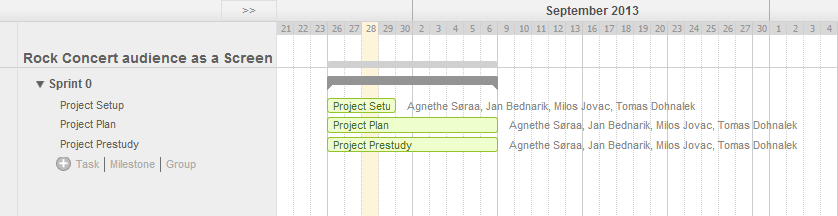
\includegraphics[scale=0.6]{images/gantt}
    \caption{Gantt Chart}
    \label{img:gantt}
\end{center}
\end{figure}

\subsection{Milestones}
\section{Risk management}

\begin{table*}\centering \ra{1.3}
    \caption{Skills}
    \label{tab:skills}
    \vspace{2mm}
    \begin{tabular}{lcccc}
    \toprule
                                & Agnethe   & Tomas & Milos & Jan \\
    \midrule
    \textbf{Leadership                 } & 4         & 1     & 2     & 3     \\ 
    \textbf{Scrum                      } & 4         & 1     & 1     & 1     \\ 
    \textbf{Mobile software development} & 3         & 1     & 4     & 1     \\ 
    \textbf{\LaTeX                     } & 1         & 4     & 1     & 4     \\ 
    \textbf{Network programming        } & 2         & 3     & 3     & 3     \\ 
    \textbf{Image processing           } & 1         & 3     & 1     & 2     \\ 
    \textbf{Java                       } & 3         & 2     & 5     & 1     \\ 
    \textbf{C++                        } & 1         & 4     & 3     & 4     \\ 
    \textbf{Testing                    } & 1         & 4     & 2     & 3     \\
    \bottomrule
    \end{tabular}
\end{table*}


\end{document}
